\documentclass{beamer}
\usepackage[utf8]{inputenc}
\usepackage[english]{babel}
\usepackage{minted}
\usepackage{comment}
%\usepackage{graphics}
\usepackage{graphicx}
%https://tex.stackexchange.com/questions/365292/how-to-use-non-ascii-chars/365303#365303
\usepackage{pmboxdraw}
\usepackage{biblatex}
\usepackage{amsmath}
\usepackage{amssymb}

\newenvironment{code}{\VerbatimEnvironment \begin{minted}{haskell}}{\end{minted}}
\newenvironment{ascii}{\VerbatimEnvironment \begin{minted}{text}}{\end{minted}}
\newcommand{\hsmint}[1]{\mintinline{haskell}{#1}}

\addbibresource{references.bib}
\begin{document}


\title{Probabilistic Programming: Use cases and implementation}
\author{Siddharth Bhat}
\institute{IIIT Hyderabad}
\date{November 16, 2019\par (FunctionalConf '19)}

\begin{frame}[fragile]
\titlepage
\end{frame}


\begin{frame}[fragile]{Outline}
    \begin{itemize}
        \item How is this different from \hsmint{System.Random}?
        \item What is Probabilistic programming, and when can I use it?
        \item A sketch of the algorithm.
        \item Hunt me down post-talk for a wealth of details.
    \end{itemize}
\end{frame}

\begin{frame}[fragile]{Our primitives}
\begin{code}
data Rand a = ...

instance Functor Rand
instance Applicative Rand
instance Monad Rand

-- | Convert a pure value into a Rand value
return :: a -> Rand a

-- | Get a random number in [0, 1)
uniform01 :: Rand Float

-- | Take `n` samples from a random variable
samples :: Int -> Rand a -> [a]

-- | take a Float, do *something*, and return no nothing
score :: Float -> Rand ()
\end{code}



\end{frame}


\begin{frame}[fragile]{First example -- The same as \hsmint{System.Random}}
\begin{columns}
\column{0.5\linewidth}
\begin{code}
-- | dice
dice :: Rand Int
dice = do
  u <- uniform01
  return $ 1 + floor (6*u)
\end{code}

\column{0.5\linewidth}
\begin{code}
-- | sum of dice
tossDice :: Rand Int
tossDice = do
    d1 <- dice
    d2 <- dice
    return $ d1 + d2
\end{code}
\end{columns}

\begin{code}
main :: IO ()
main = do
  print $ sample 10 tossDice
  drawHistogram $ sample 100 tossDice
\end{code}

\textbf{Output:}
\input{"| cabal v2-exec slides -- tossDice"}
\end{frame}


\begin{frame}[fragile]{Raytracing (Default)}
\begin{columns}
\column{0.2\linewidth}
        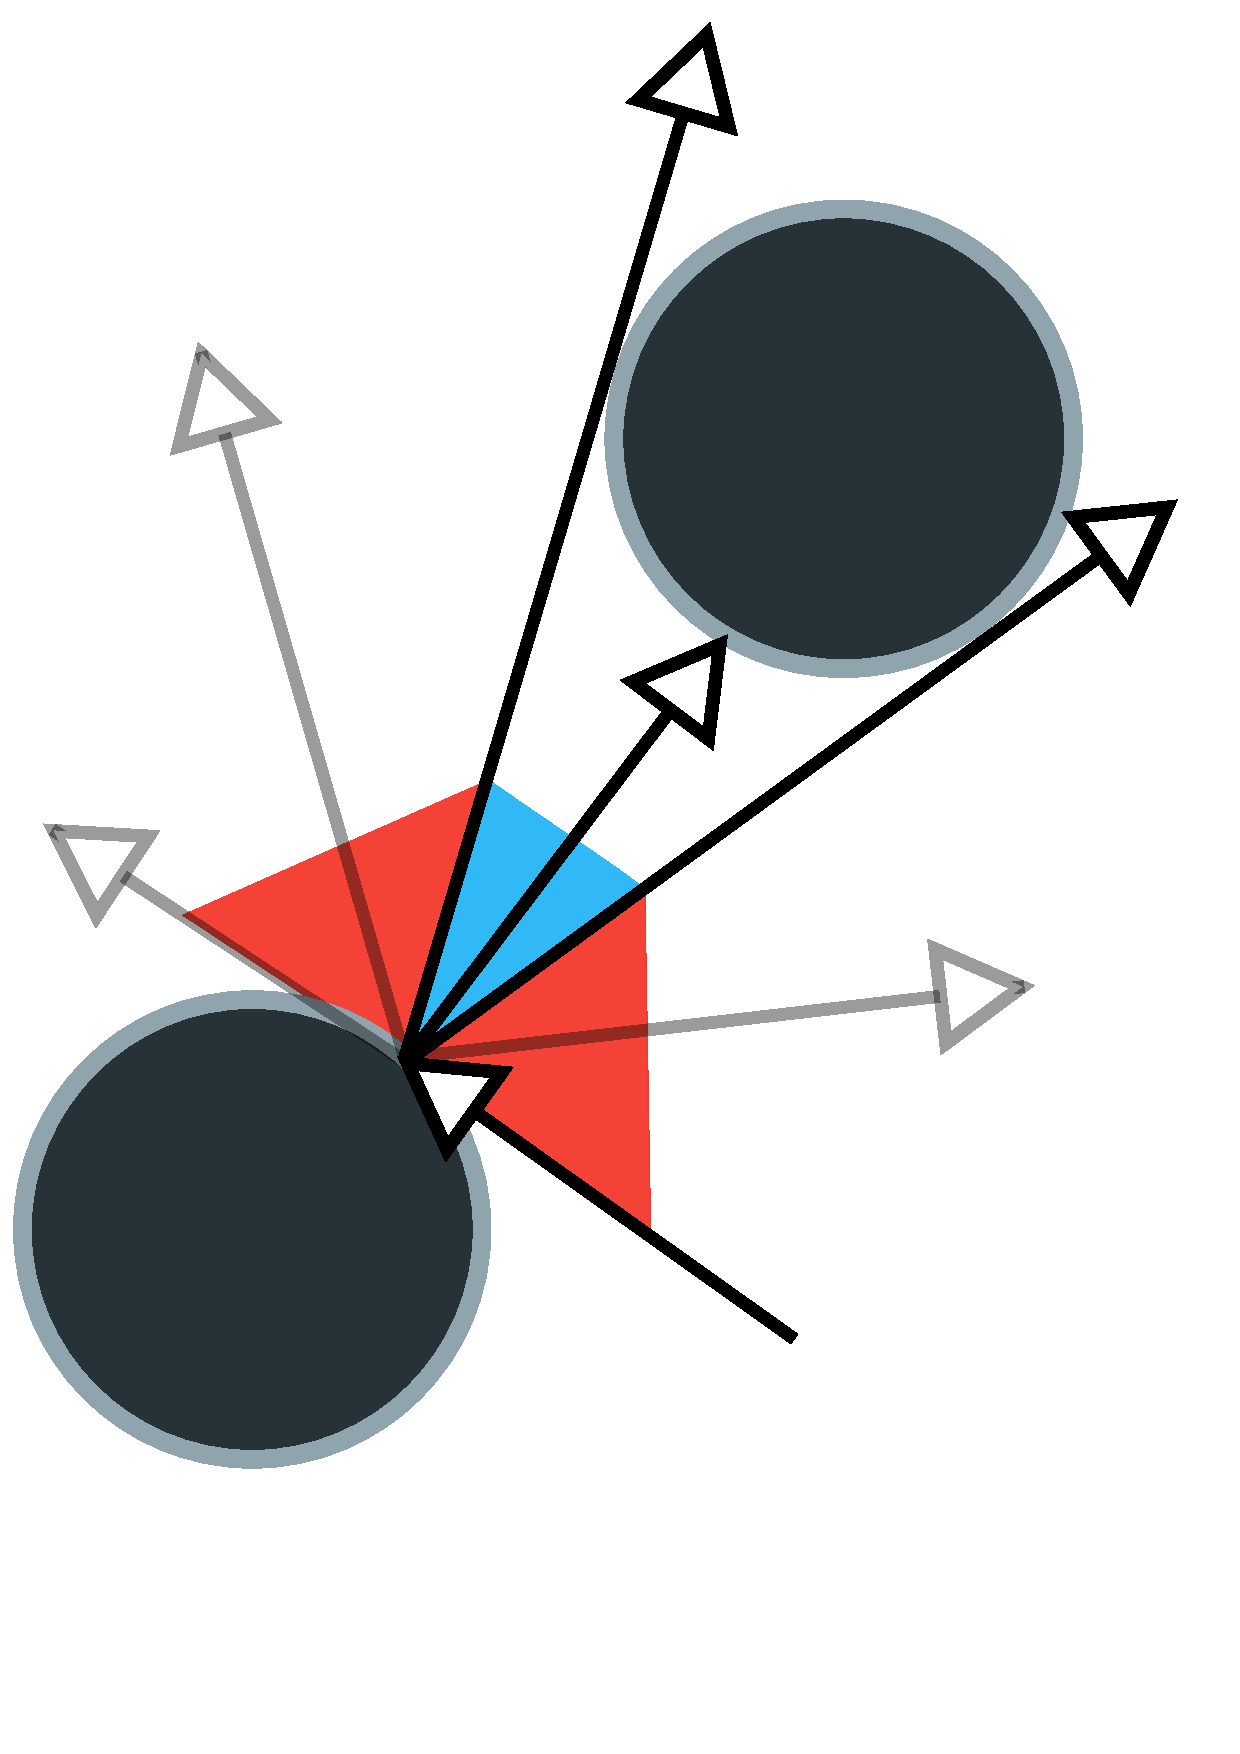
\includegraphics[height=180px]{res/raytrace.pdf}
\column{0.6\linewidth}
{\scriptsize
\begin{code}
  -- | recursively raytrace
  raytrace :: Ray -> Rand Color
  raytrace r = do
    case getCollision r of
      Some (surface, loc) -> 
       color' <- averageRays loc
       return $ mixColor surface color'
      None -> return backgroundColor

  -- | Send a random ray 
  sendRandRay :: Position -> Rand Color
  sendRandRay p =
    u <- uniform01
    let angle = 360 * u
    raytrace (makeRay p angle)

  -- | Average rays sent from a location
  averageRays :: Position -> Rand Color
  averageRays p = do
    -- | computationally wasteful
    colors <- replicateM 100 (sendRandRay p)
    return $ averageColors colors

  -- | Default background color.
  backgroundColor = white
\end{code}
}
\end{columns}
\end{frame}

\begin{frame}[fragile]{Raytracing (Scored)}
\begin{columns}
\column{0.5\linewidth}
{\scriptsize
\begin{code}
  raytrace :: Ray -> Rand Color
  raytrace r = do
    case getCollision r of
      Some (surface, loc) -> 
       color' <- averageRays loc
       return $ mixColor surface color'
      None -> return backgroundColor
\end{code}
}

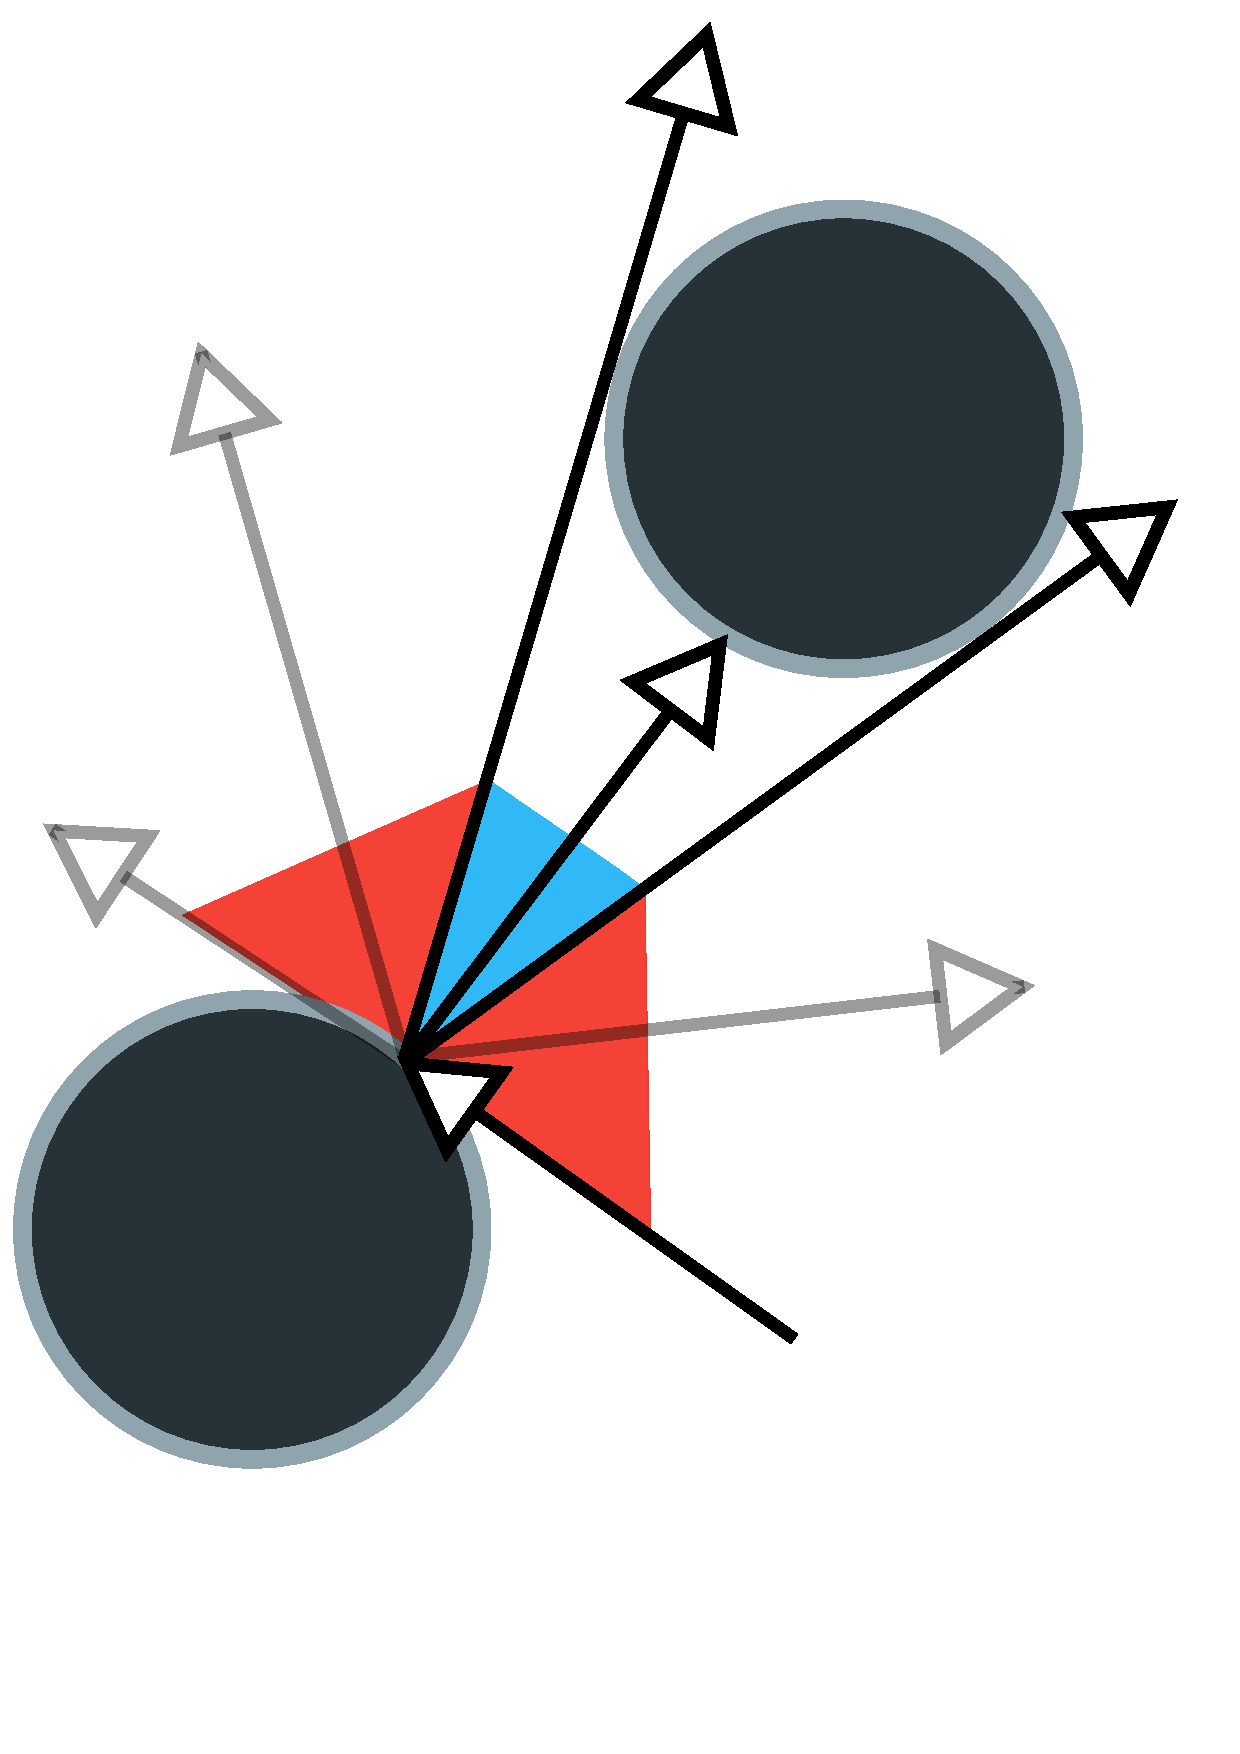
\includegraphics[height=180px]{res/raytrace.pdf}

\pause
\column{0.5\linewidth}
{\scriptsize
\begin{code}
  raytrace' :: Ray -> Rand Color
  raytrace' r = do
    case getCollision r of
      Some (surface, loc) -> 
       color' <- averageRays loc
       return $ mixColor surface color'
      None -> do
        score 0.5 -- New! 
        return backgroundColor
\end{code}
}
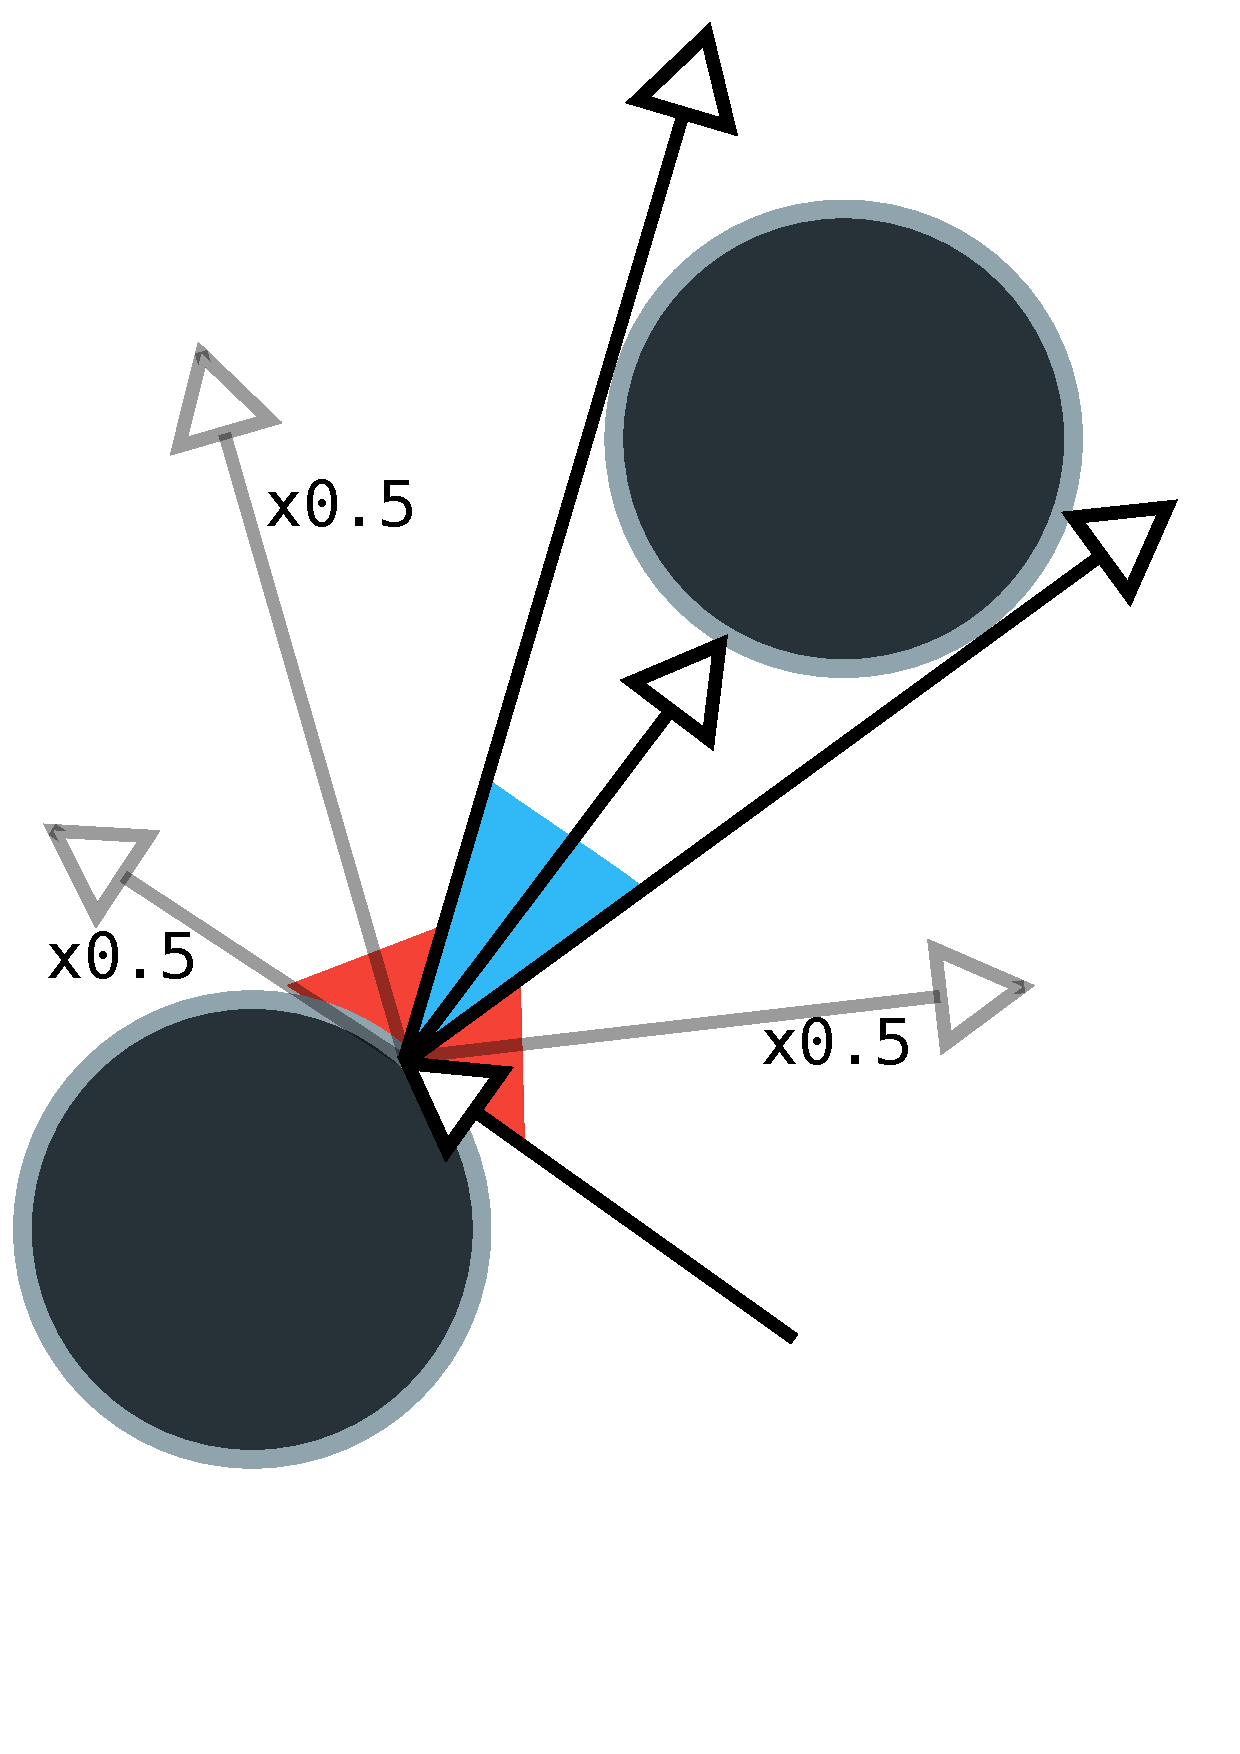
\includegraphics[height=180px]{res/raytrace-scored.pdf}
\end{columns}
\end{frame}

\begin{frame}[fragile]{Exploring a complicated landscape}

\begin{code}
-- | Naive understanding / Little knowledge when we begin
prior :: Rand a
prior = ...

-- | Learn as you go!
learn :: Rand a
learn = do
  value <- prior
  score (usefulness value)
  return value

-- | Generate samples according to unknown distribution
-- (Rays from the raytracing)
landscape :: [a]
landscape = samples 1000 learn

\end{code}
\end{frame}


\begin{frame}[fragile]{Program optimisation}
\begin{itemize}
\item A hypothetical stack-based machine (eg. JVM bytecode!)
\item Instructions are \texttt{Push}, \texttt{Add}, \texttt{Dup}, \texttt{Sub}

\begin{ascii}
f(x) = x*2
Program(f) = [Push 2; Mul]
[BOT x] -Push 2-> [BOT x; 2] -Mul-> [BOT x*2]
\end{ascii}
\pause
\item Want to automatically discover optimizations
\begin{ascii}
f(x) = x*2 = x+x
Program(f) = [Dup; Add]
[BOT x] -Dup-> [BOT x; x] -Add-> [BOT x+x]
\end{ascii}
Faster (addition is faster than multiplication)
\pause
\item Neural nets do not work - no gradient $\frac{\partial loss}{\partial program}$
\end{itemize}
\end{frame}

\begin{frame}[fragile]{Program optimization pseudocode (Random)}
Key idea: Randomly change the initial program and pick the best.
\begin{columns}
\column{\linewidth}
{\scriptsize \footnotesize
\begin{code}
-- | Randomly change programs and return their performance
equivRandomProgram :: Program -> Rand (Performance, Program)
equivRandomProgram p = do
  p' <- modifyProgram p
  if semanticsEqual p p'
  then return (performance p', p')
  else return (0, p') -- A program that does not work has 0 perf.

-- | Take the random samples and pick the good performing ones
optimise :: Program -> Program
optimise p = 
  let ps' = sample 100 (equivRandomProgram p)
  in snd $ maximumBy (\a b -> compare (fst a) (fst b)) ps'
\end{code}
}
\end{columns}
\end{frame}


\begin{frame}[fragile]{Program optimisation pseudocode (Scored)}
\begin{columns}
\column{\linewidth}
{\scriptsize \footnotesize
\begin{code}
equivRandomProgram :: Program -> Rand (Performance, Program)
equivRandomProgram p = do
  p' <- modifyProgram p
  if semanticsEqual p p'
  then return (performance p', p')
  else return (0, p') -- A program that does not work has 0 perf.
\end{code}
\pause
\begin{code}
equivRandomProgram' :: Program -> Rand (Performance, Program)
equivRandomProgram' p = do
 (perf, p) <- equivRandomProgram p
 let perf = 
    if semanticsEqual p p'
      then 5 + performance p' -- Correct programs are given high score
      else performance p' -- Fast incorrect programs are also allowed
 score perf -- ^ Correct programs are more likely
 return (perf, p')
\end{code}
}

{\scriptsize \tiny
    \texttt{http://stoke.stanford.edu/}\qquad
    \texttt{https://github.com/bollu/blaze/blob/master/notebooks/tutorial.ipynb}
}
\end{columns}
\end{frame}

\begin{frame}[fragile]{Transformations discovered by \texttt{STOKE}}
\begin{columns}
\column{\linewidth}
{\scriptsize
\begin{itemize}
\item
\begin{ascii}
f = 2 + 3
(nparams: 0 | [IPush 2,IPush 3,IAdd])
\end{ascii}
\pause
\begin{ascii}
[IPush 5] | score: 2.5
// constant folding: 2 + 3 -> 5
\end{ascii}
\pause

\item
\begin{ascii}
f(x) = 2 * x
(nparams: 1 | [IPush 2,IMul])
\end{ascii}
\pause
\begin{ascii}
[IDup,IAdd] | score: 2.25 
// strength reduction: 2 * x -> x + x
\end{ascii}
\pause

\item
\begin{ascii}
f(x) = x & x
(nparams: 1 | progInsts = [IDup,IAnd])
\end{ascii}
\pause
\begin{ascii}
[] | score: 3.0
// algebraic rewrite: x & x == x
\end{ascii}
\end{itemize}
}
\end{columns}
\end{frame}

\begin{frame}[fragile]{\texttt{STOKE}: The intuition}
    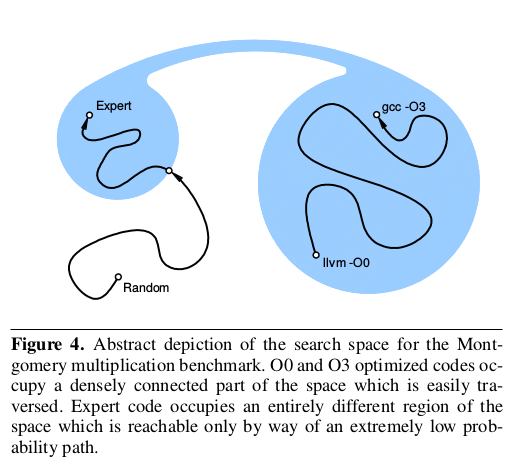
\includegraphics[width=256px]{res/MCMC-STOKE.png}
\end{frame}


\begin{frame}[fragile]{\texttt{STOKE}: The intuition}
    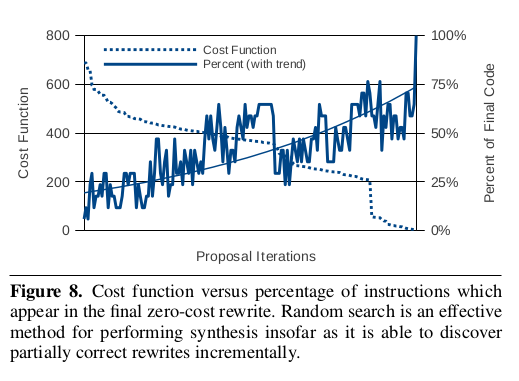
\includegraphics[width=256px]{res/STOKE-why-random-search-works.png}
\end{frame}

\begin{frame}[fragile]{\texttt{STOKE}: A real-world example}
    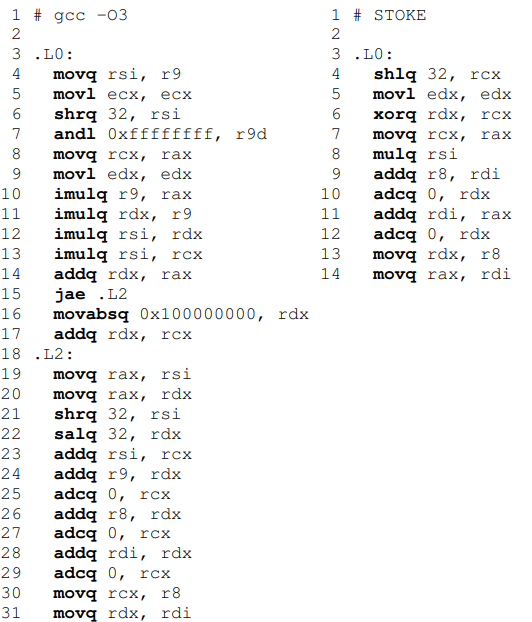
\includegraphics[height=200px]{res/STOKE-real-world-code.png}
\end{frame}

\begin{frame}[fragile]{Gradient-free optimisation on a complicated landscape}

\begin{code}
-- | Naive understanding / Little knowledge when we begin
prior :: Rand a
prior = ...

-- | Learn as you go!
learn :: Rand (Score, a)
learn = do
  value <- prior
  let s = score (usefulness value)
  return (s, value)

-- | Sample and pick best value (random programs)
-- | Works because sampler will "move" towards 
-- scored regions!
best :: (Score, a)
best = maximumBy (\a b -> compare (fst a) (fst b))
        (samples 1000 learn)
\end{code}

\end{frame}



\begin{frame}[fragile]
\begin{code}
data Rand x where
    Ret :: x -> Rand x
    SampleUniform01 :: (Double -> Rand x) -> Rand x
    Score :: Float -> Rand x -> Rand x

instance Functor Rand
instance Applicative Rand
instance Monad Rand
\end{code}
(\hsmint{Rand} is a free monad)
\begin{code}
return :: x -> Rand x
return = Ret

uniform01 :: Rand Float
uniform01 = SampleUniform01 Ret

score :: Float -> Rand ()
score s = Score s (return ())
\end{code}
\end{frame}

\begin{frame}[fragile]
\begin{code}
-- | Run the computation _unweighted_,
-- | ignores scores.
sampleUnweighted :: RandomGen g => g -> Rand a -> (a, g)
sampleUnweighted g (Ret a) = (a, g)
sampleUnweighted g (SampleUniform01 f2my) =
  let (f, g') = random g in sample g' (f2my f)
sampleUnweighted g (Score f mx) = 
  error "unable to handle Score"
\end{code}
\end{frame}


\begin{frame}[fragile]{Semantics of Score: Uniform probability}
    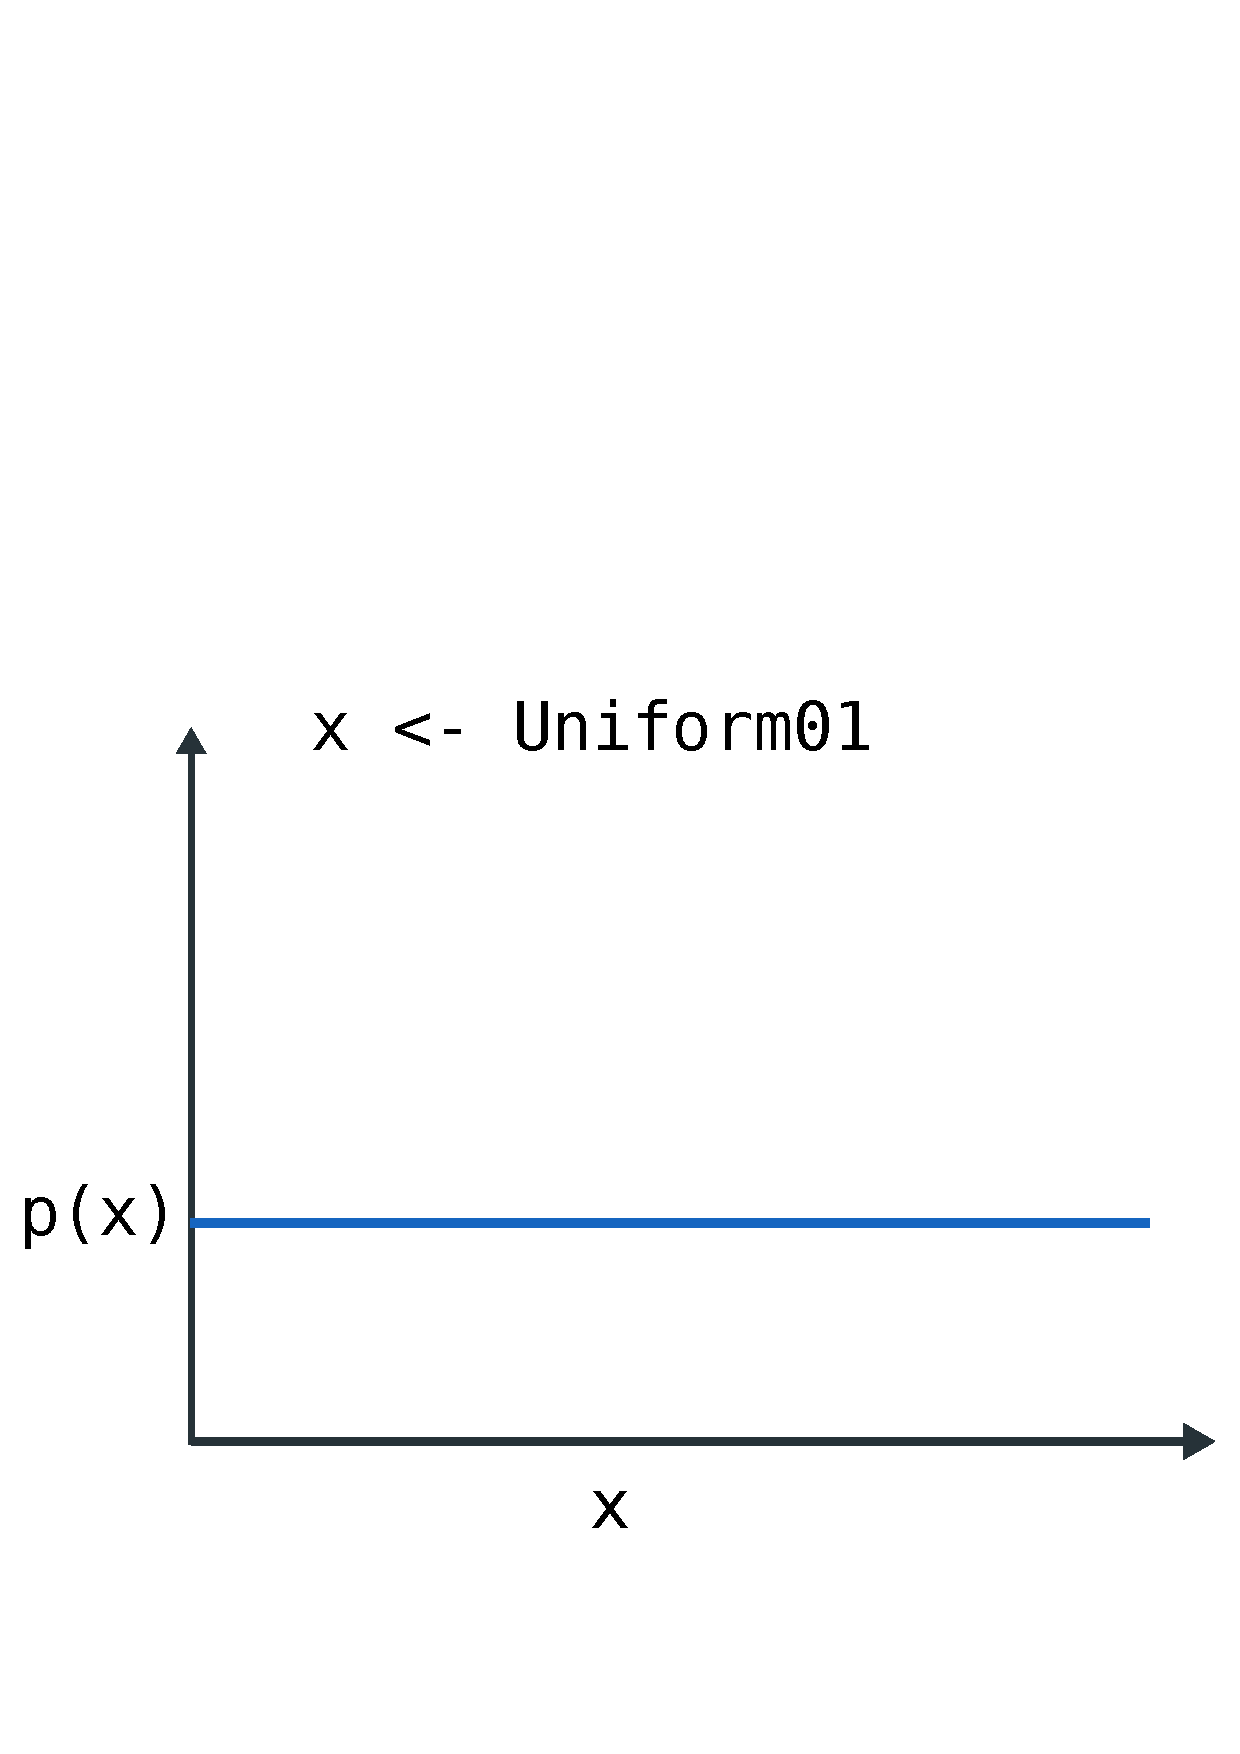
\includegraphics[height=280px]{res/uniform-PDF.pdf}
\end{frame}

\begin{frame}[fragile]{Semantics of Score: Custom ratios of probabilities!}
    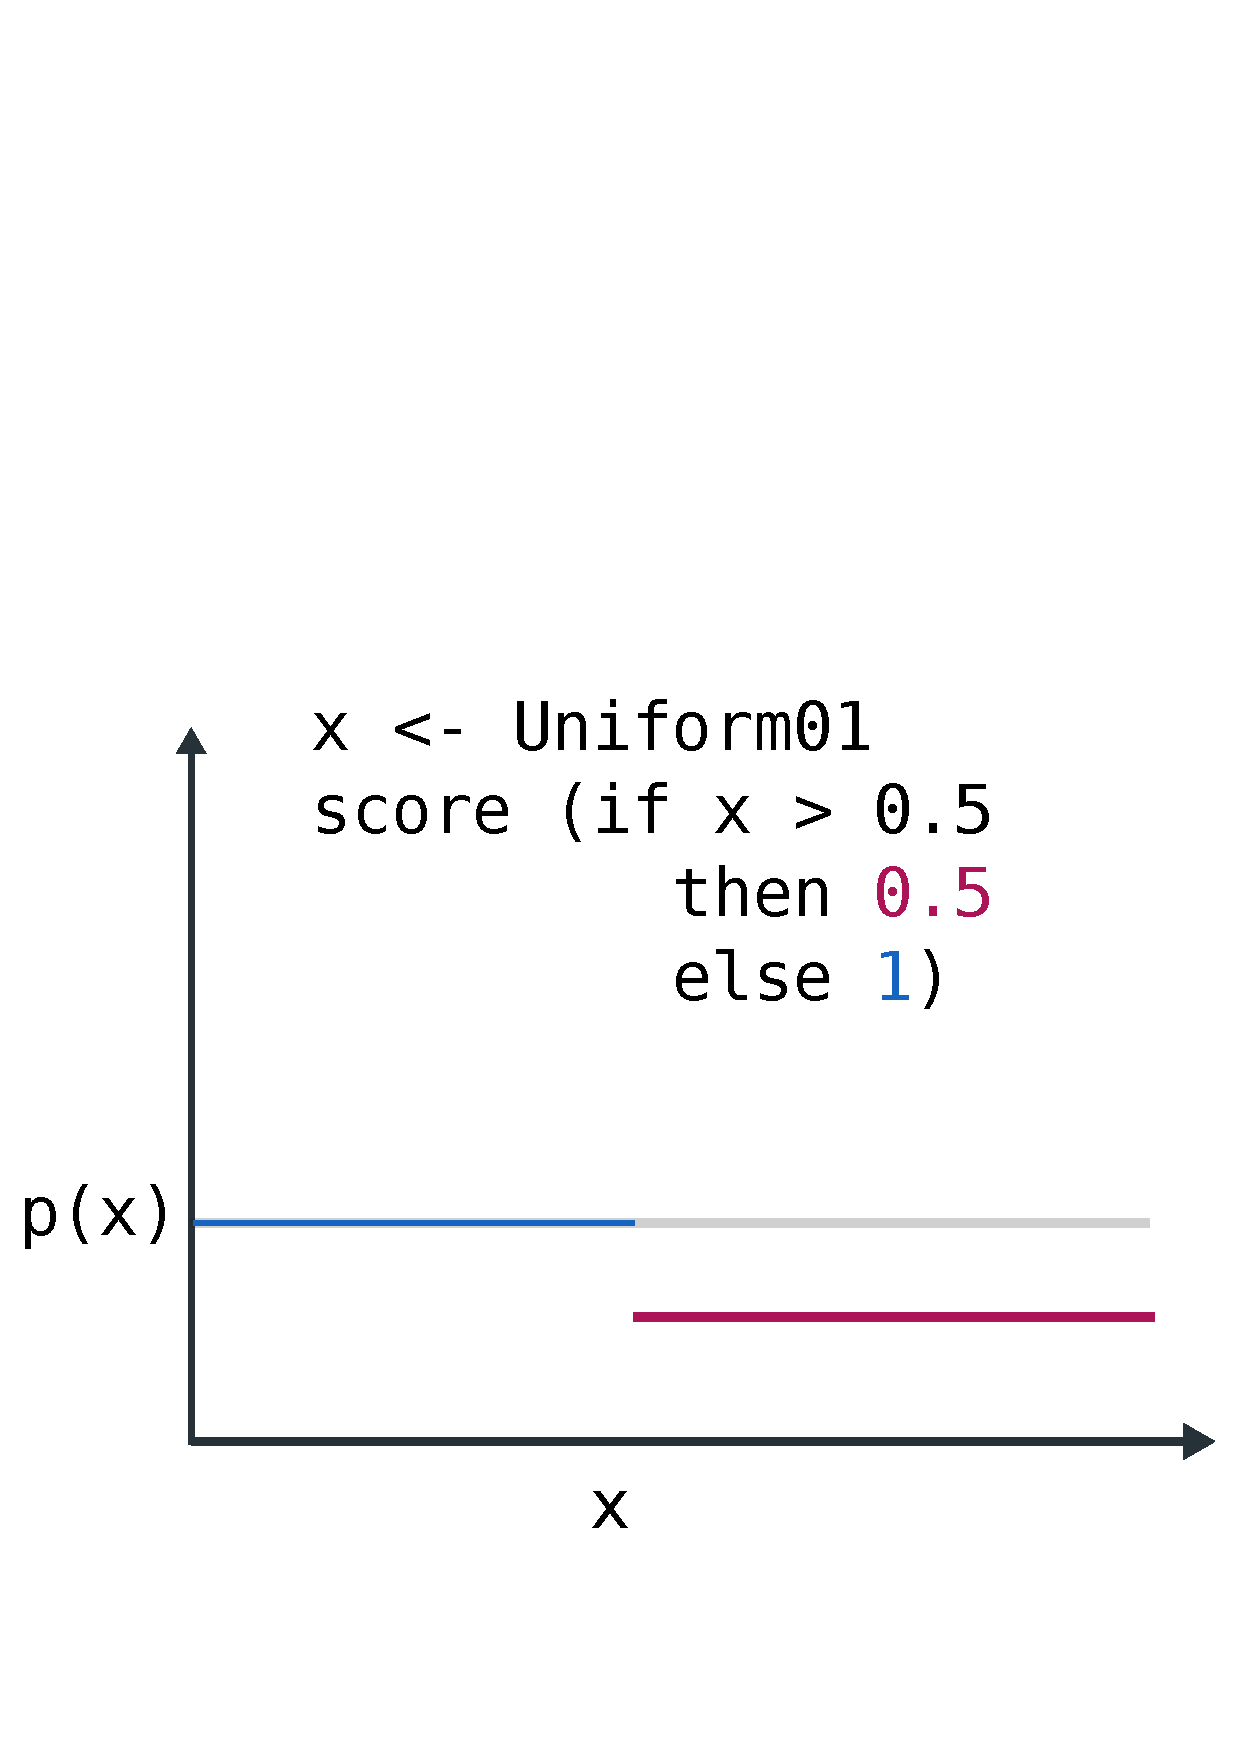
\includegraphics[height=280px]{res/MCMC-1.pdf}
\end{frame}

\begin{frame}[fragile]{How do we handle Score?}
    \begin{itemize}
        \item Game plan: convert \hsmint{Rand a} to \hsmint{Rand (Trace a)}.
        \item \hsmint{Rand a} may contain \hsmint{Score}, \hsmint{Rand (Trace a)} will not.
        \item \hsmint{Rand (Trace a)} will have extra information to make \hsmint{Score} work.
        \item Can use \hsmint{sampleUnweighted} on \hsmint{Rand (Trace a)}. It will respect \hsmint{Score}, but not use \hsmint{Score}.
\end{itemize}
\end{frame}

\begin{frame}[fragile]{Traced Computations - Program}
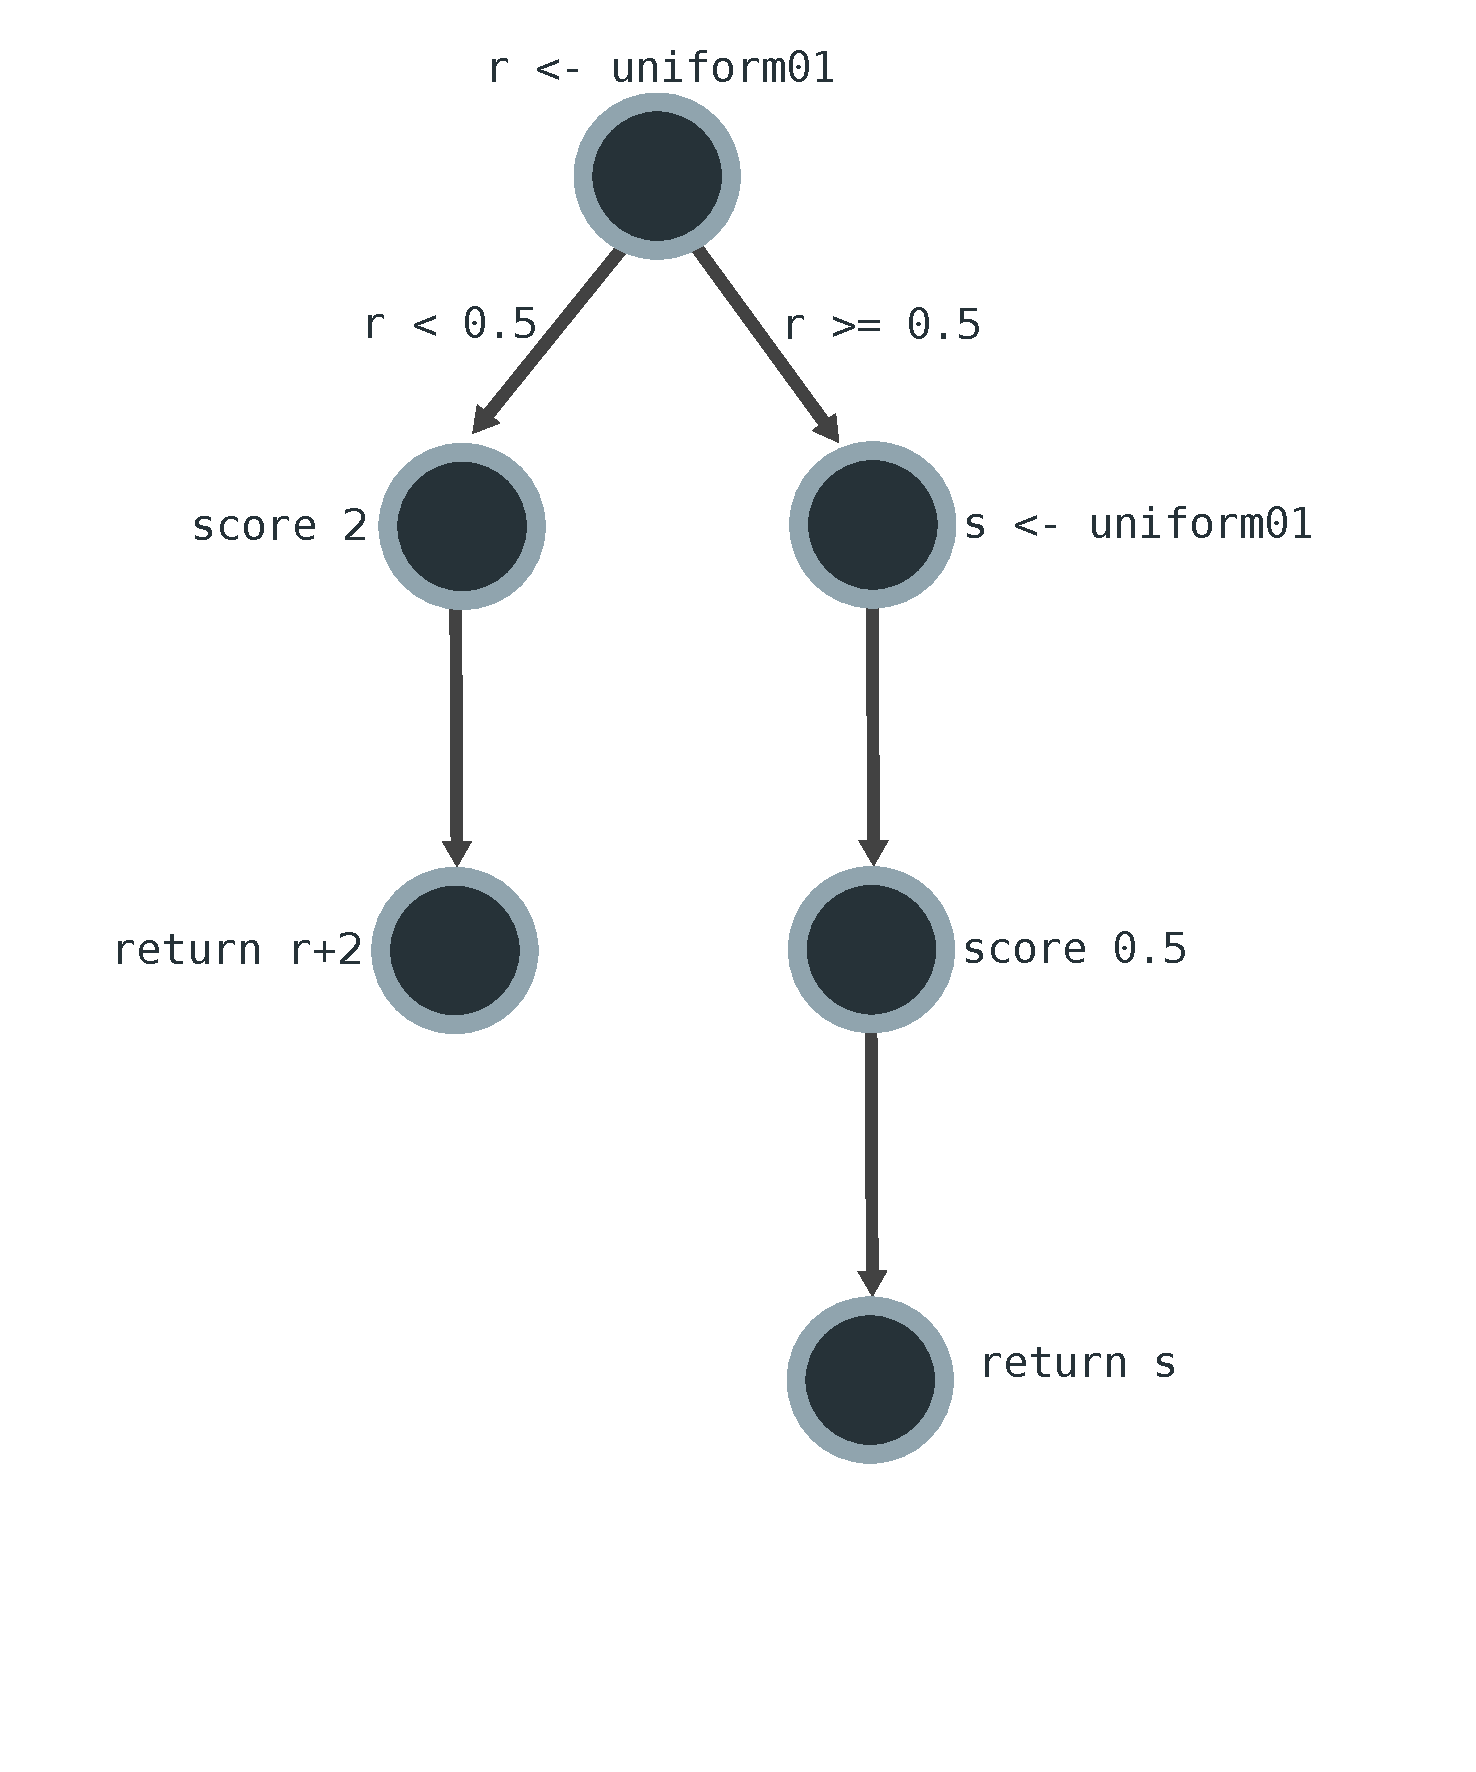
\includegraphics[height=280px]{res/program-1.pdf}
\end{frame}

\begin{frame}[fragile]{Traced Computations - Trace 1}
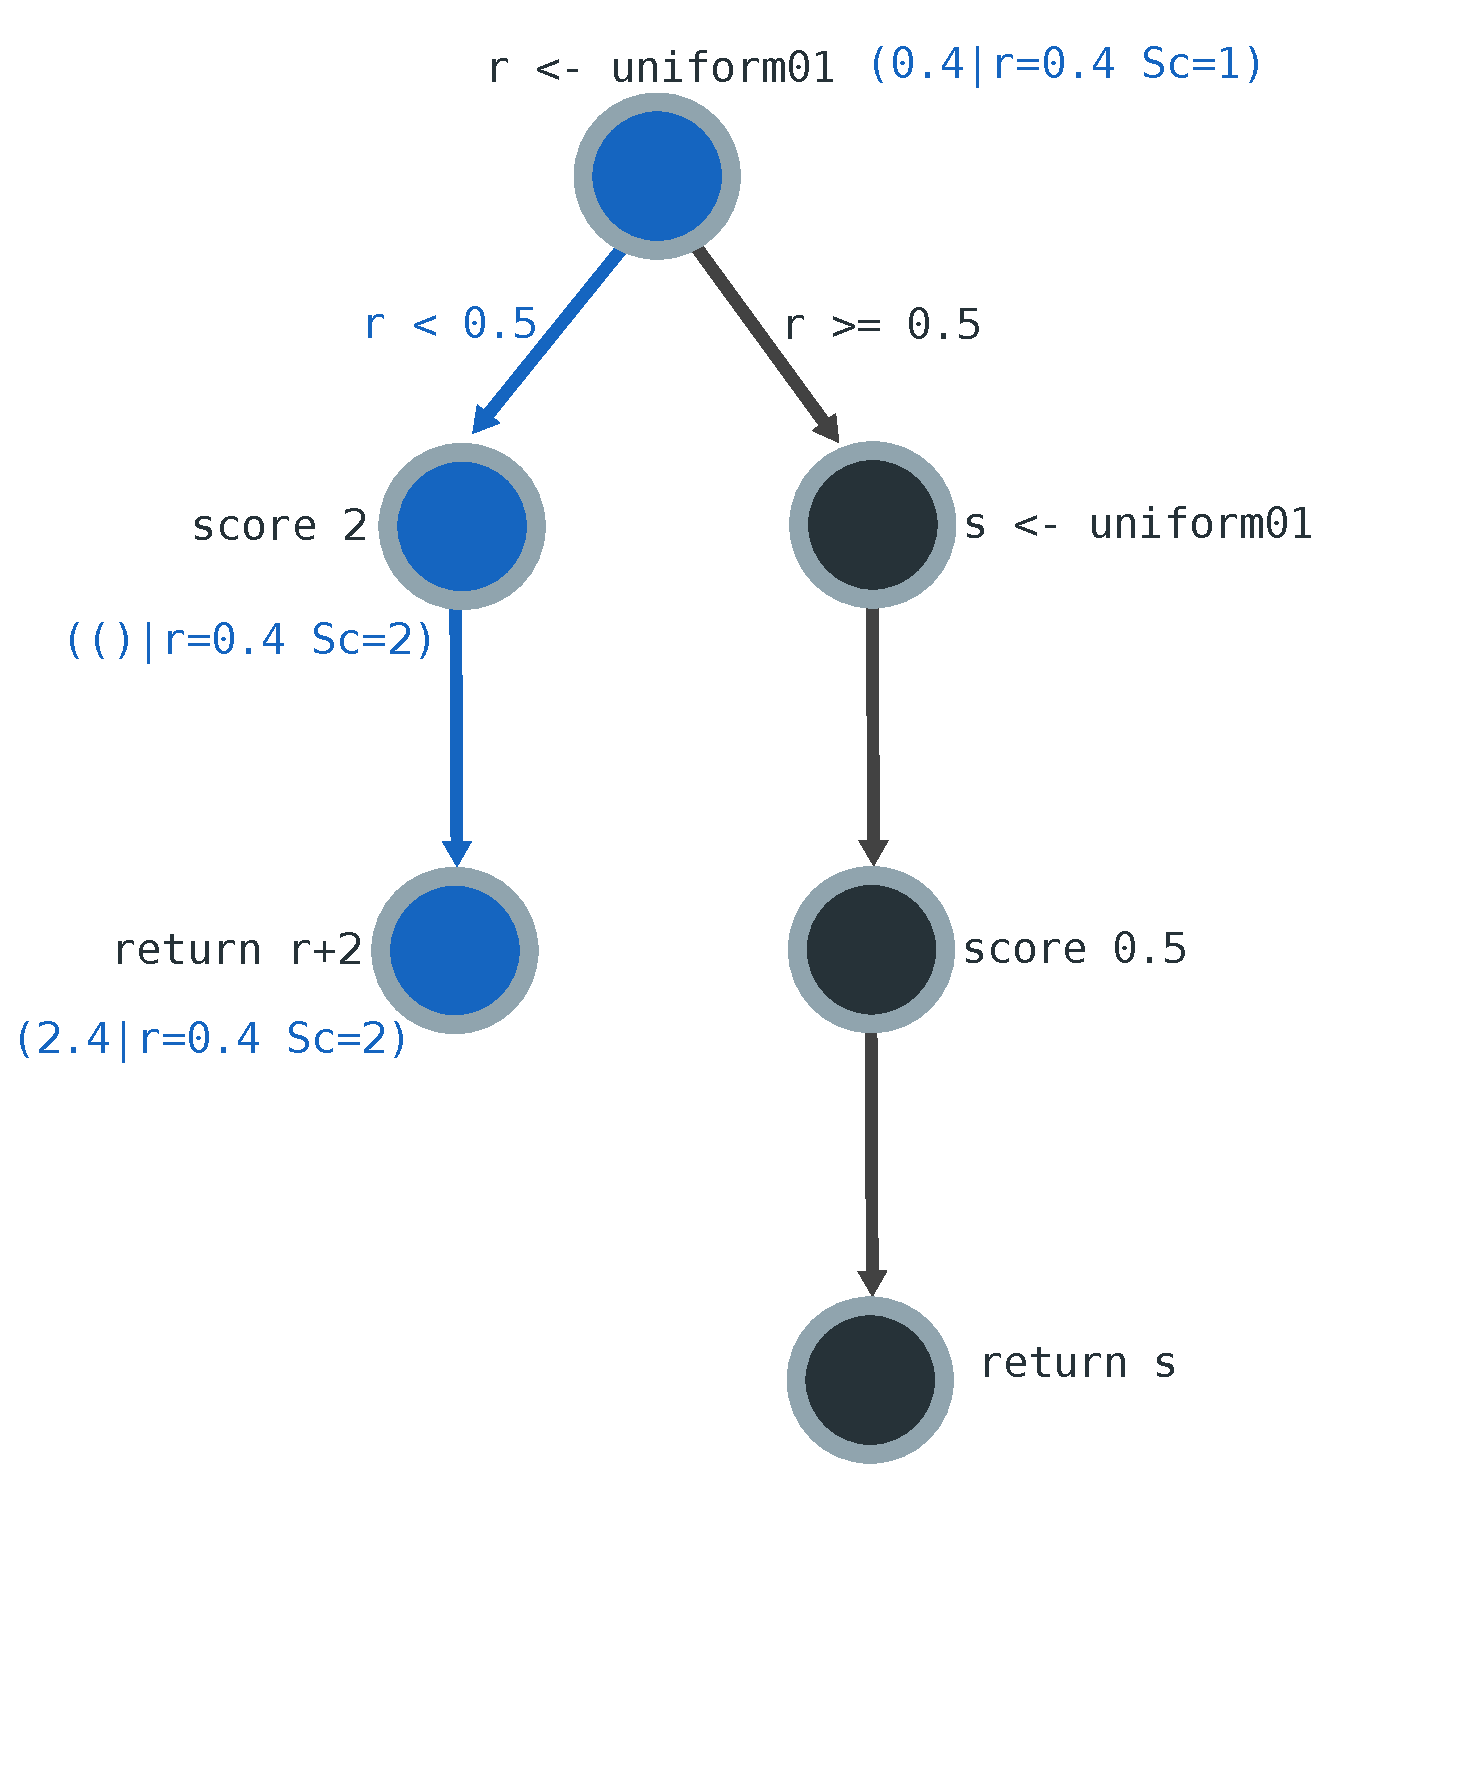
\includegraphics[height=280px]{res/program-2.pdf}
\end{frame}


\begin{frame}[fragile]{Traced Computations - Trace 2}
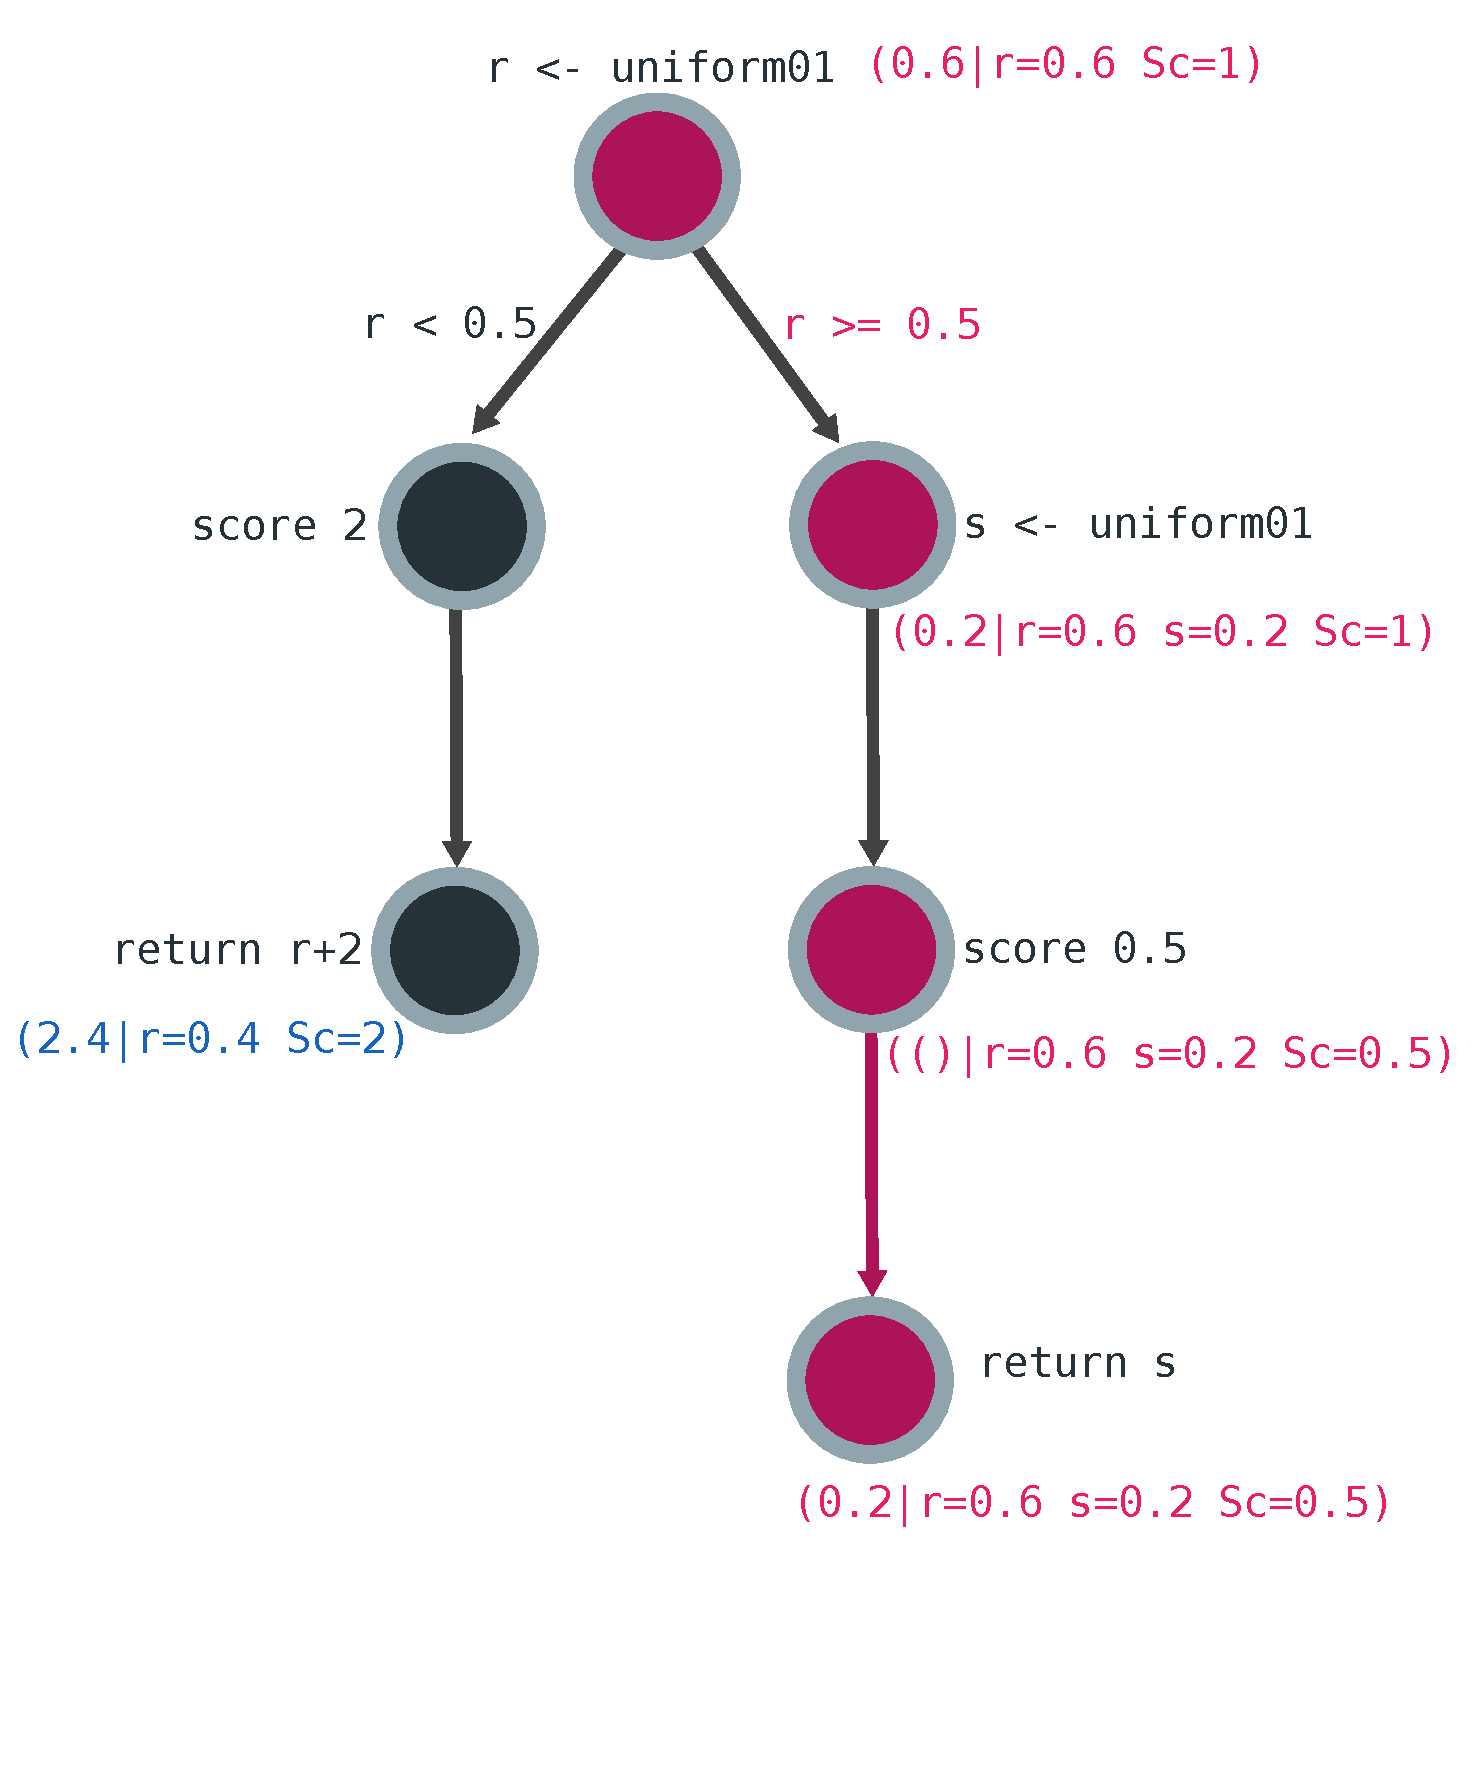
\includegraphics[height=280px]{res/program-3.pdf}
\end{frame}


\begin{frame}[fragile]{Traced Computations - Trace 3}
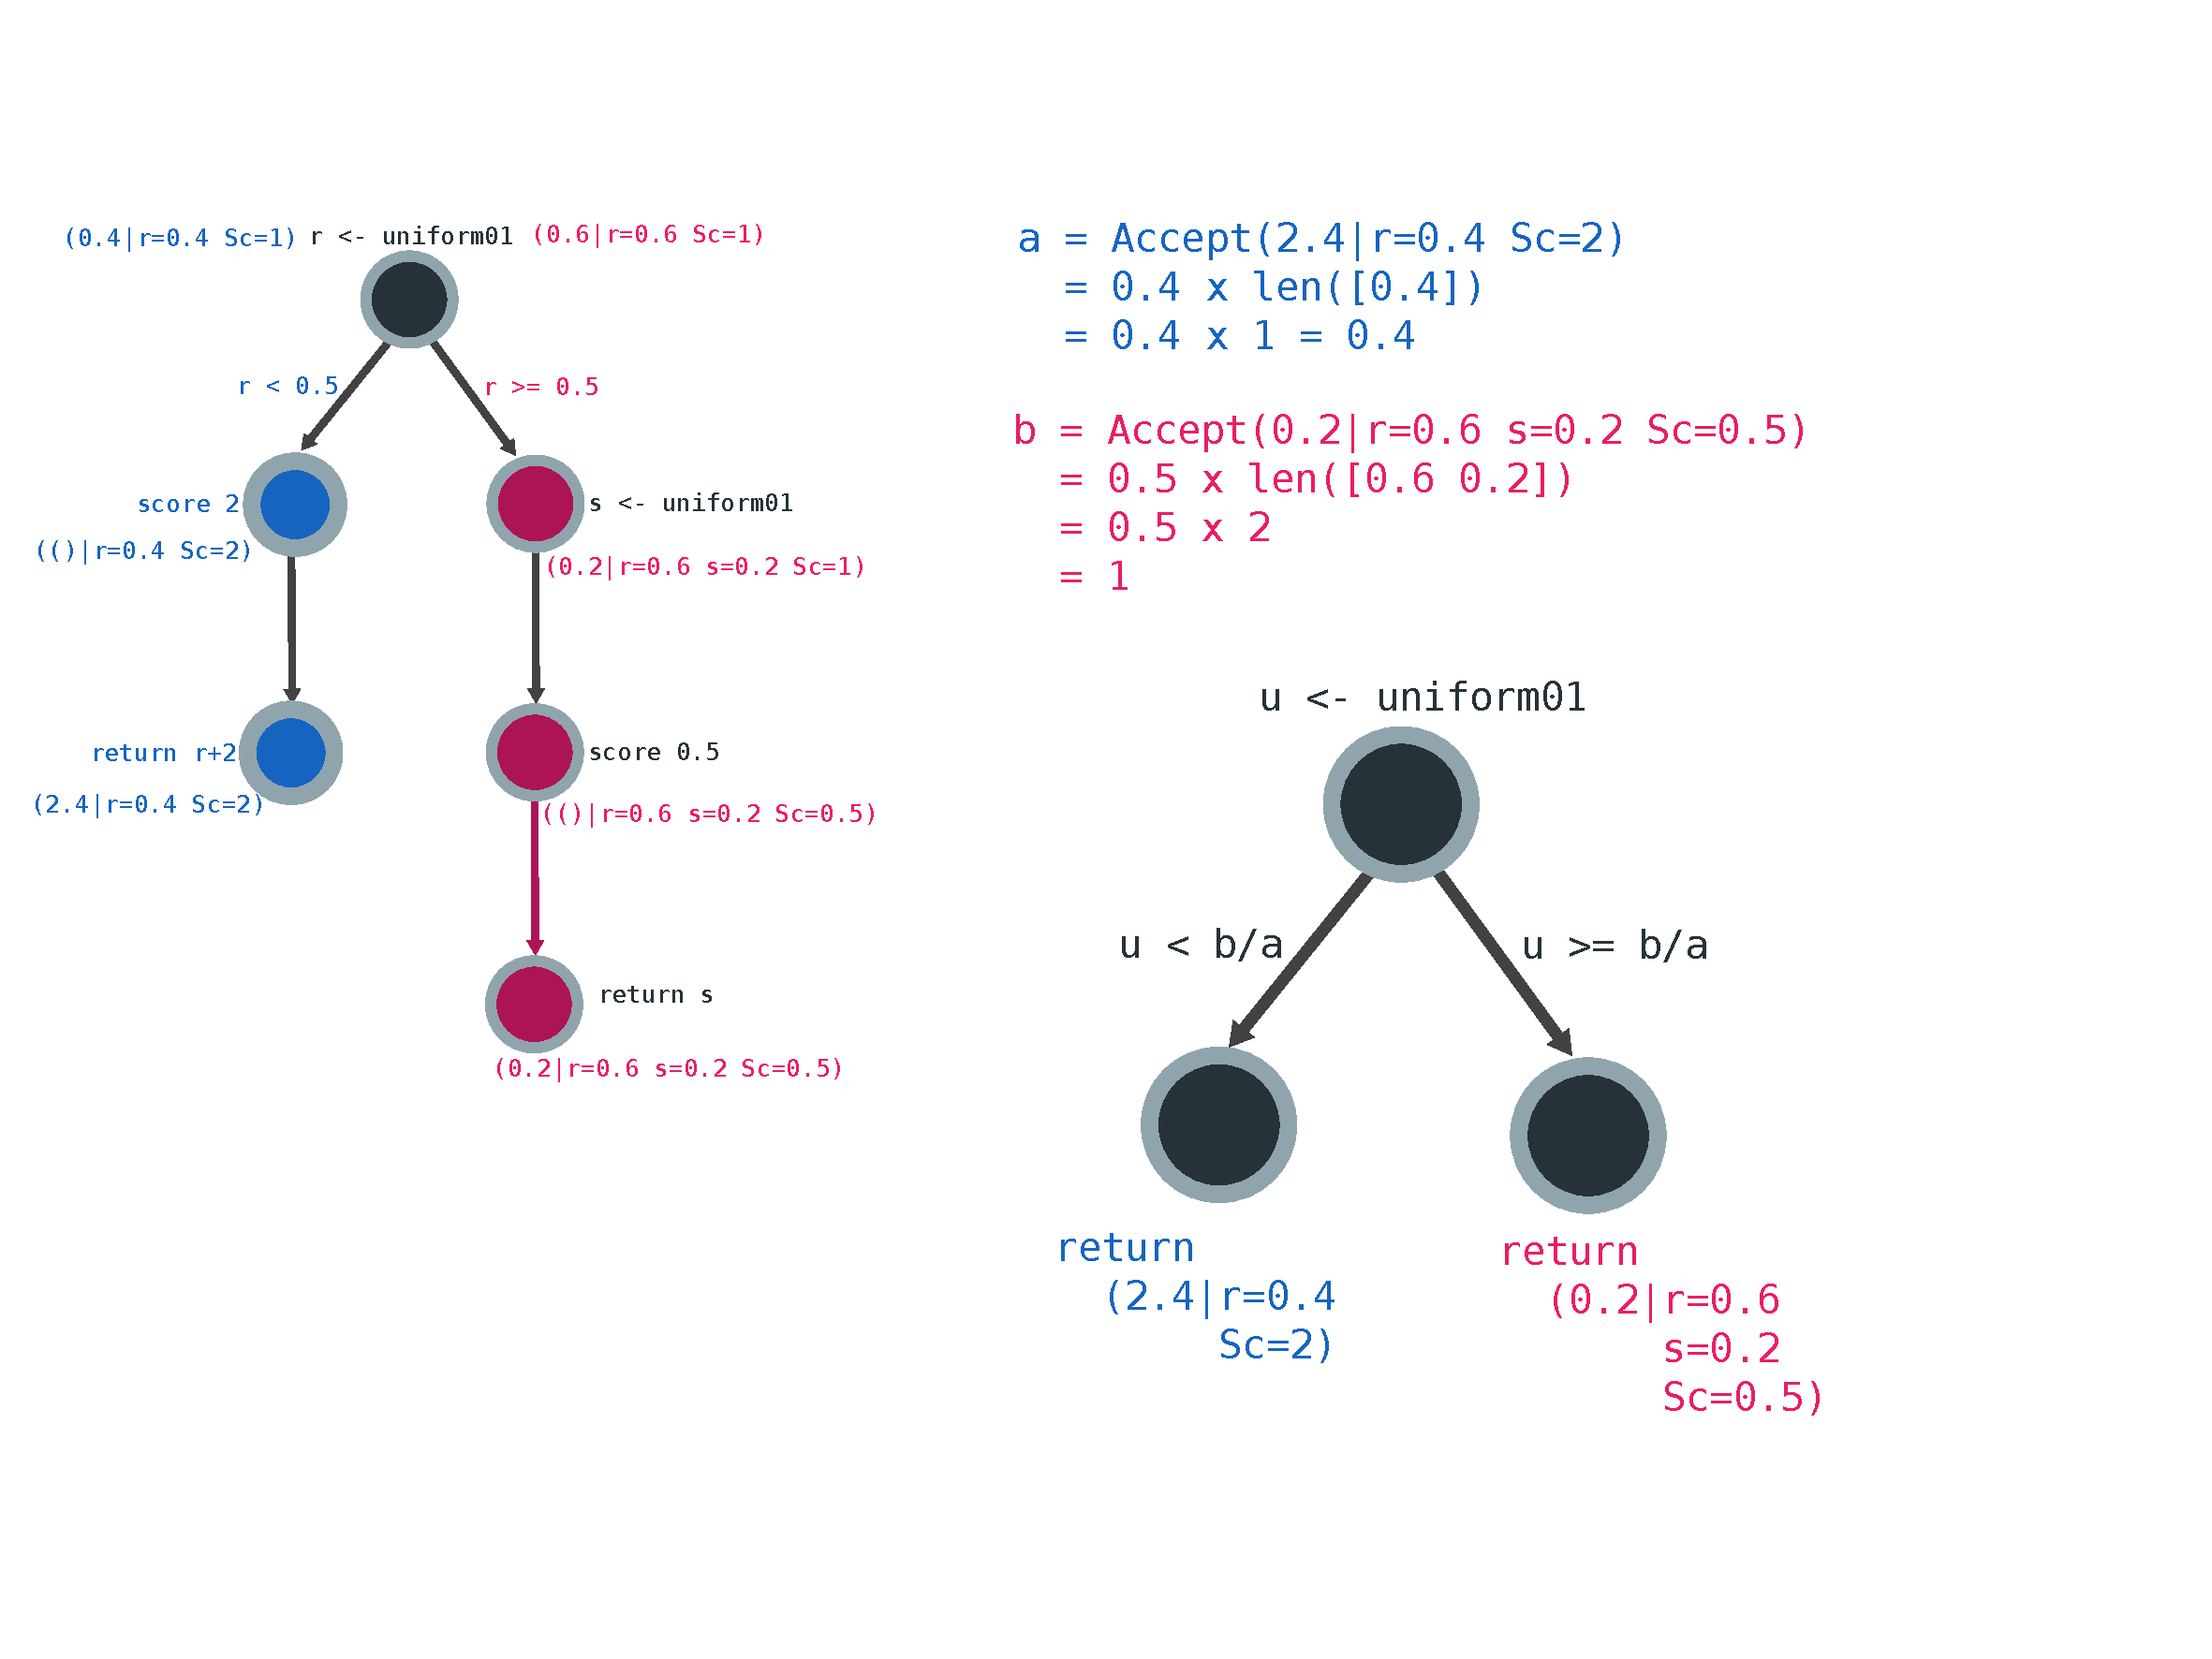
\includegraphics[height=280px]{res/program-4.pdf}
\end{frame}


\begin{frame}[fragile]{Tracing: the data structure}
\begin{columns}
\column{\linewidth}
{
\begin{code}
-- | Trace all random choices made
data Trace a =
  Trace { tval :: a, -- ^ The value itself
          tscore :: Double, -- ^ The total score
          trs :: [Double] -- ^ The random numbers used
        }
\end{code}
}
\end{columns}
\end{frame}


\begin{frame}[fragile]{Introspection of a Free monad}
\begin{columns}
\column{\linewidth}
%\column{0.5\linewidth}
%\column{0.5\linewidth}
{\scriptsize
\begin{code}
-- | Trace a random computation (remove Score)
traceR :: Rand x  -- ^ Original computation
  -> Rand (Trace x) -- ^ Traced computation
traceR (Ret x) = Ret (Trace x 1.0 [])
traceR (SampleUniform01 mx) = do
  r <- sample01
  trx <- traceR $ mx r
  return $ trx { trs=trs ++ [r]}
traceR (Score s mx) = do -- ^ No score in the RHS
  trx <- traceR $ mx
  return $ trx { tscore = tscore*s}
\end{code}
}
\pause
{\scriptsize
\begin{code}
-- | Send a particular sequence of randomness
feedRandomness :: [Float] -- ^ Randomness to use
  -> Rand a -- ^ Original computation
  -> Rand a -- ^ Fixed computation
feedRandomness _ (Ret x) = Ret x
feedRandomness 
  (r:rs) (SampleUniform01 f) = 
    feedRandomness rs (f r)
feedRandomness rs (Score s plx) = 
  Score s $ injectRandomness rs plx
\end{code}
}
\end{columns}
\end{frame}


\begin{frame}[fragile]{Metropolis Hastings}
\begin{code}
mhStep :: Rand (Trace x) -- ^ proposal
         -> Trace x -- ^ current position
         -> Rand (Trace x) -- ^ new
mhStep r trace = do
  -- | Return the original randomness, perturbed
  rands' <- perturbRandomness (trs trace)
  -- | Run the original computation with the perturbation
  trace' <- feedRandomness rands' r
  let ratio = trAccept trace' / trAccept trace
  r <- sample01
  return $ if r < ratio then trace' else trace
\end{code}
  
\begin{columns}
\column{0.5\linewidth}
{\scriptsize
\begin{code}
trAccept :: Trace x -> Double
trAccept tx =
  tscore tx * 
  fromIntegral (length (trs tx))
\end{code}
}
\column{0.5\linewidth}
{\scriptsize
\begin{code}
perturbRandomness :: [Double] 
  -> Rand [Double]
perturbRandomness rands = do
  -- | Random index
  ix <- choose [0..(length rands-1)]
  r <- sample01 -- ^ random val
  -- | Replace random index
  -- with random val.
  return $ replaceListAt ix r rands 
\end{code}
}
\end{columns}
\end{frame}




\begin{frame}[fragile]{Odds and Ends}
\begin{columns}
\column{\linewidth}
{\scriptsize
\begin{code}
-- | run the computation after taking weights into account
samples :: Int -> Rand x -> Rand [x]
samples 0 _ = return []
samples n r =
  let tracedR = traceR r
      -- go :: Int -> Rand (Trace x) -> Rand (Trace [x])
      go 0 _ = return []
      go n tx = do
        tx' <- repeatM 10 (mhStep tracedR) $ tx -- !
        txs <- go (n-1) tx'
        return (tx:txs)
  in do
      seed <- findNonZeroTrace $ tracedR
      tracedRs <- go n seed 
      return $ map tval tracedRs
\end{code}
}
\end{columns}

\begin{columns}
\column{\linewidth}
{\scriptsize
\begin{code}
-- | Find a starting position that does not have probability 0
findNonZeroTrace :: Rand (Trace x) -> Rand (Trace x)
findNonZeroTrace tracedR = do
  trace <- tracedR
  if tscore trace /= 0
  then return $ trace
  else findNonZeroTrace tracedR
\end{code}
}
\end{columns}

\end{frame}

\begin{frame}[fragile]{Takeaways}
    \begin{itemize}
        \item Probabilistic Programming is a powerful model of computation.
        \item Free monads is essential: allows for introspection.
        \item Implementation is deceptively simple (hopefully!)
    \end{itemize}
\end{frame}

\begin{frame}[fragile]{Thank you!}
  \begin{beamercolorbox}[center]{title}
    Questions?
  \end{beamercolorbox}





  \vfill
  \begin{beamercolorbox}[center]{title}
        
\includegraphics[height=64px]{res/tweag-io.pdf}
  \end{beamercolorbox}

  \begin{beamercolorbox}[center]{title}
    (A huge thank you to everyone at \texttt{tweag.io} who read the literature with me!)
  \end{beamercolorbox}
\end{frame}


\begin{frame}[allowframebreaks]{References}
        %\bibliographystyle{acm}
        %\bibliographystyle{amsalpha}
        \nocite{*}
        \printbibliography
\end{frame}


\begin{frame}[fragile]{Use case: Bayesian updates}
\begin{code}
predictCoinBias :: [Int] -> Rand Double
predictCoinBias flips = do
  b <- sample01
  forM_ flips $ \f -> do
    -- | Maximum a posterior
    score $ if f == 1 then b else (1 - b)
  return $ b
\end{code}

\begin{code}
predictCoinBiasNoData :: Rand Double
predictCoinBiasNoData = predictCoinBias []
\end{code}

\input{"| cabal v2-exec slides -- predictCoinBiasNoData"}


\begin{code}
predictCoinBias0 :: Rand Double
predictCoinBias0 = predictCoinBias [0]
\end{code}

\input{"| cabal v2-exec slides -- predictCoinBias0"}

\begin{code}
predictCoinBias01 :: Rand Double
predictCoinBias01 = predictCoinBias [0, 1]
\end{code}

\input{"| cabal v2-exec slides -- predictCoinBias01"}

\end{frame}


\begin{frame}[fragile]{Use case: Sample from arbitrary distributions}

\begin{code}
sampleSinSq :: Rand Double
sampleSinSq = do
  x <- (6 *) <$> sample01
  score $ (sin x) * (sin x)
  return $ x
\end{code}

\input{"| cabal v2-exec slides -- sampleSinSq"}

\end{frame}


\begin{frame}{Deep dive into MCMC methods}
\end{frame}

\begin{frame}[fragile]{Probability Distributions: the tension}
    \begin{columns}
        \column{0.5\linewidth}
        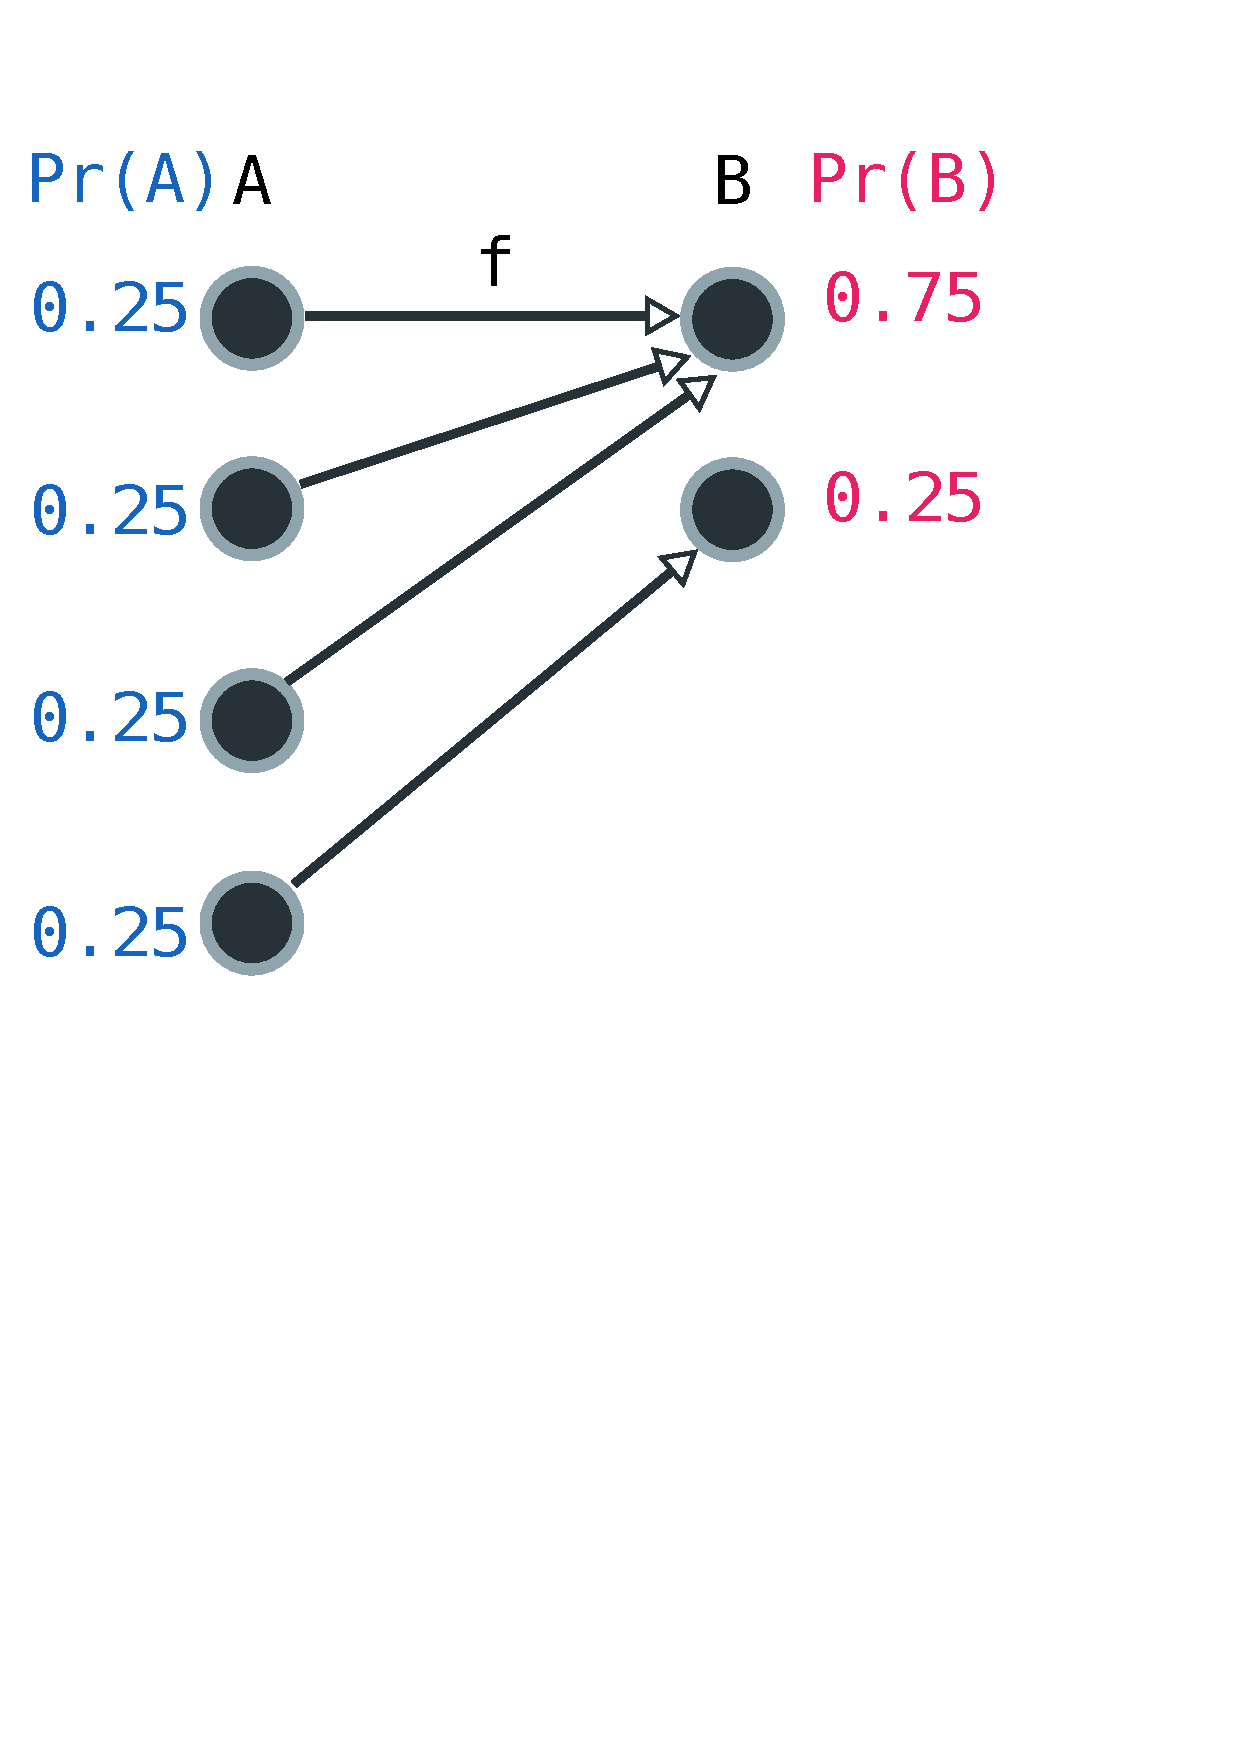
\includegraphics[height=256px]{res/density-forward.pdf}
        \column{0.5\linewidth}
        \begin{itemize}
            \item $f: A \rightarrow B$ is known.
            \item $f^{-1}: B \rightarrow A$ is required for the density.
            \item This is intractable.
        \end{itemize}
    \end{columns}
\end{frame}





\end{document}


